\chapter{Background}\label{chap:background}
\section{The Mass Balancing Problem}

\begin{figure}
    \centering
    \usetikzlibrary{arrows.meta,3d}
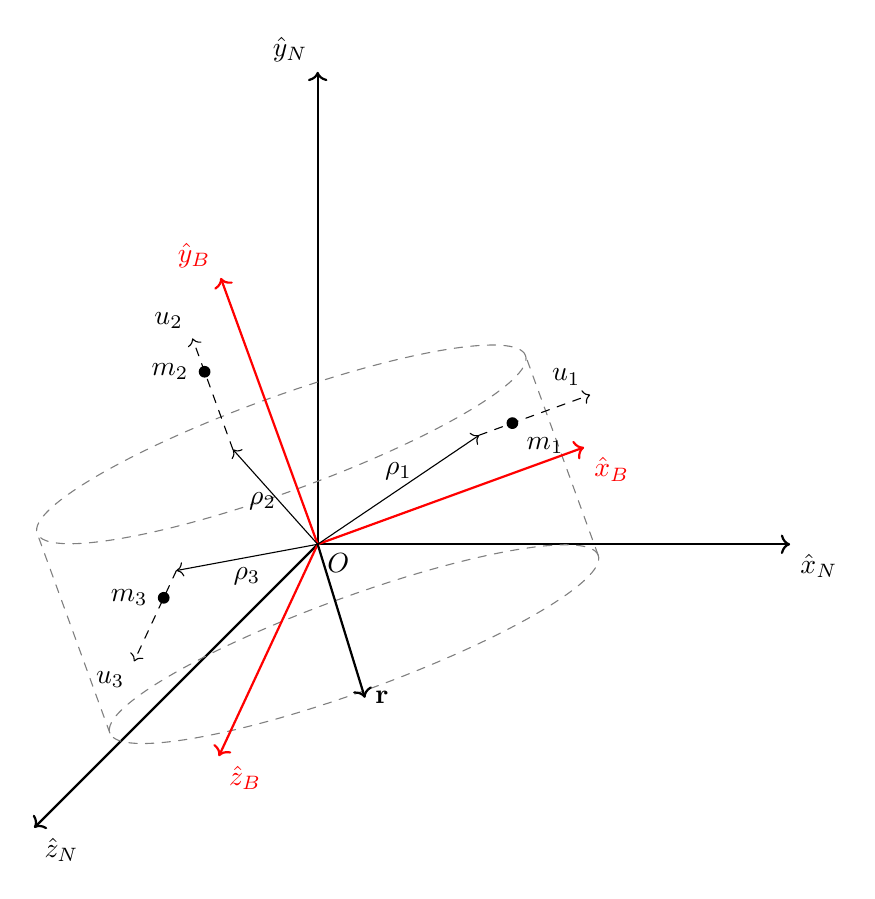
\begin{tikzpicture}[scale=3, line cap=round, line join=round]

% Inertial frame (I)
\draw[->, thick] (0,0) -- (2,0) node[below right] {$\hat{x}_N$};
\draw[->, thick] (0,0) -- (0,2) node[above left] {$\hat{y}_N$};
\draw[->, thick] (0,0) -- (-1.2,-1.2) node[below right] {$\hat{z}_N$};
\node[below right] at (0,0) {$O$};

% Cylinder representing platform ------------------------------
\pgfmathsetmacro{\radius}{1.1}
\pgfmathsetmacro{\height}{0.9}

\begin{scope}[rotate around={20:(0,0)}] 
    \draw[gray,dashed] (0,-\height/2) ellipse ({\radius} and 0.2);
    \draw[gray,dashed] (0,\height/2) ellipse ({\radius} and 0.2);
    \draw[gray,dashed] (-\radius,-\height/2) -- (-\radius,\height/2);
    \draw[gray,dashed] (\radius,-\height/2) -- (\radius,\height/2);
\end{scope} 

% Body frame (B), shifted and rotated
\begin{scope}[rotate=20]
    \draw[->, thick, red] (0,0) -- (1.2,0) node[below right] {$\hat{x}_B$};
    \draw[->, thick, red] (0,0) -- (0,1.2) node[above left] {$\hat{y}_B$};
    \draw[->, thick, red] (0,0) -- (-0.7,-0.7) node[below right] {$\hat{z}_B$};
    % \node[below left, red] at (0,0) {$\mathcal{B}$};

    % START M2 --------------------------------------
    \draw[->] (0,0) -- (-0.2,0.5) coordinate (rho2_end) 
        node[pos=0.65, below] {$\rho_2$};

    \draw[->, dashed] (rho2_end) -- ++(0,0.5) coordinate (u2_end)  
        node[above left] {$u_2$};

    \path (rho2_end) -- (u2_end) 
        node[pos=0.7, circle, fill=black, inner sep=1.5pt, label=left:$m_2$] {};

    % START M1 --------------------------------------
     \draw[->] (0,0) -- (0.8,0.2) coordinate (rho1_end) 
        node[midway, above] {$\rho_1$};

    \draw[->, dashed] (rho1_end) -- ++(0.5,0) coordinate (u1_end)  
        node[above left] {$u_1$};

    \path (rho1_end) -- (u1_end) 
        node[pos=0.3, circle, fill=black, inner sep=1.5pt, label=below right:$m_1$] {};

    % START M3 -----------------------------------
    \draw[->] (0,0) -- (-0.6,0.1) coordinate (rho3_end) 
        node[midway, below] {$\rho_3$};

    \draw[->, dashed] (rho3_end) -- ++(-0.3,-0.3) coordinate (u3_end)  
        node[below left] {$u_3$};

    \path (rho3_end) -- (u3_end) 
        node[pos=0.3, circle, fill=black, inner sep=1.5pt, label=left:$m_3$] {};
\end{scope}

% START COM r ----------------------------------
\draw[->, thick] (0,0) -- (0.2, -0.65) coordinate (r_end)
    node[below, right] {$\mathbf{r}$};
 




\end{tikzpicture}
    \caption{The mass balancing problem for air bearing based spacecraft dynamics simulators}
    \label{fig:mbs_problem}
\end{figure}


\Cref{fig:mbs_problem} defines the geometery of the problem in a general case. $O$ represents the common origin of the inertial frame $\mathcal{N}$ and the body-fixed principle frame of the simulator $\mathcal{B}$. $O$ is chosen to by the center of rotation . If frictionless rotation is assumed, then the simulator follows Euler's rotational equations of motion with gravity acting as a torque. 

\begin{equation}
    \bm{J}\,\dot{\bm{\omega}} + \bm{\omega}^{\times}\,\bm{J}\bm{\omega} = \bm{T}_g
\end{equation}

Here, $\bm{J}$ is the inertia of the simulator about $O$, $\bm{\omega}$ is the angular velocity of the simulator, and $\bm{T}_g$ is the torque due to gravity. $\dot{\bm{v}}$ represents the time derivative of some vector $\bm{v}$, and $\bm{v}^{\times}$ represents the skew-symmetric cross-product matrix of $\bm{v}$. All vectors and inertias are expressed in $\mathcal{B}$. In general it is more convienent to expand $\bm{T}_g$ which leads to

\begin{equation}\label{equation:starting_eom}
    \bm{J}\,\dot{\bm{\omega}} + \bm{\omega}^{\times}\,\bm{J}\bm{\omega} = m_s\bm{r}^{\times}\bm{g}
\end{equation}

where $m_s$ is the total mass of the simulator, $\bm{r}$ is the center of mass relative to $O$, and the $\bm{g}$ is the accleration due to gravity.

\Cref{fig:mbs_problem} also shows the introduction of three sliding masses, although in general there may be as many as $n$ sliding masses. Each mass $m_i$ has one translational degree of freedom along $\bm{u}_i$, and $\bm{\rho}_i$ represents the position of the $i$-th mass in it's zeroed position. Since in practice each mass can only travel some limited distance along $\bm{u}_i$, the zeroed position of a mass is defined as the center of this range of positions. The position relative to $O$ of any mass $\bm{R}_i$ can be obtained with 
\begin{equation}\label{equation:sliding masses}
    \bm{R}_i = \bm{\rho}_i + d_i\bm{u_i}
\end{equation}
where $d_i$ is the distance a mass $m_i$ has travelled along $u_i$ relative to it's zeroed position. In a more most general case, $\Delta\,d_i$ is defined as the change in position a mass from any arbitrary starting position.

The goal of these definitions is to obtain an equation relating how changing the positions of each mass effects the center of mass of the total system. These parameters are first assembled into matricies as follows

\begin{equation}
    \bm{M}=\mathrm{diag}(\frac{m_1}{m_s}, \cdots  ,\frac{m_n}{m_s}) \in \mathbb{R}^{n \times n}
\end{equation}
\begin{equation}
    \bm{U}=
    \begin{bmatrix}
        \bm{u}_1, & \cdots & ,\bm{u}_n
    \end{bmatrix}
    \in \mathbb{R}^{3 \times n}
\end{equation}
\begin{equation}
    \Delta\bm{d}=
    \begin{bmatrix}
        \Delta\,d_1, & \cdots & ,\Delta\,d_n 
    \end{bmatrix}^T
    \in \mathbb{R}^{n}
\end{equation}

Using these defintions, writing $\Delta\bm{r}$ as a function of $\Delta\bm{d}$ becomes a simple matrix multiplication

\begin{equation}
    \Delta\bm{r} = \bm{U}\bm{M}\Delta\bm{d}
\end{equation}
 
The more important relation however is writing $\Delta\bm{d}$ as a function of $\Delta\bm{r}$. For the case $n = 3$ with linearly independent values of $\bm{u}_i$, the unique solution is given by
\begin{equation}\label{equation:delta_d_sol}
    \Delta\bm{d} = (\bm{U}\bm{M})^{-1}\Delta\bm{r}
\end{equation}
If $n>3$, a solution that minimizes the mass moved can be found using a pseudoinverse approach
\begin{equation}\label{equation:delta_d_pseudo_sol}
    \Delta\bm{d} = (\bm{U}\bm{M})^{\dagger }\Delta\bm{r}
\end{equation}

where $(\bm{U}\bm{M})^{\dagger}$ represents the Moore-Penrose pseudoinverse of $\bm{UM}$.

There are two main approaches to solving the mass balancing problem. The first is to hold the mass positions constant and obtain an estimate of the value of $\bm{r}$, denoted as $\hat{\bm{r}}$. The required change in positions of the sliding masses are then applied all at once. The exact values are calculated from \Cref{equation:delta_d_sol} or \Cref{equation:delta_d_pseudo_sol}, substituting $-\hat{\bm{r}}$ for $\Delta\bm{r}$. This class of approaches is referred to passive balancing, offline balancing, or the batch estimation method.

The second main approach is to use $\Delta\bm{d}$ as a control input. Referring to \Cref{equation:starting_eom}, the dynamics of the system are influenced by the value of $\bm{r}^{\times}$, whose value can be controlled by $\Delta\bm{d}$ using \Cref{equation:delta_d_sol} or \Cref{equation:delta_d_pseudo_sol}. The goal then becomes to find a feedback control law the drives the effect of the $m_s\bm{r}^{\times}\bm{g}$ term in \Cref{equation:starting_eom} to zero. This class of approaches is referred to as active balancing or feedback control balancing.

Once any balancing procedure has been performed, it is important to verify the results through an external verification method. Assuming the center of mass is below the center of rotation, a very rough estimate for the torque due to gravity may be obtained by tilting the simulator about one of it's principal axes, releasing it, and observing the period of resulting pendulum motion $T$ \cite{kim_automatic_2009}. The relationship between $\bm{r}$ and $T$ is given by
\begin{equation}
    T = 2\pi\sqrt{\frac{J_i}{m_s\,g||\bm{r}||}}
\end{equation}
where $J_i$ is the moment of inertia about said principle axis. After performing a balancing procedure, the value of $||\bm{r}||$ should decrease, leading to longer periods of oscillatation. 

Another verification method is observing the total mechanical energy of the simulator while it undergoes this same pendulum motion. The mechanical energy is given by
\begin{equation}
    E_{mech} = \frac{1}{2}\bm{\omega}^T\bm{J}\bm{\omega} + mgh
\end{equation}
where $h$ is the vertical height of $\bm{r}$ \cite{silva_filtering_2018}. If the simulator is balanced, $h$ will remain relatively constant throughout the pendulum motion, and the kinetic energy term $\frac{1}{2}\bm{\omega}^T\bm{J}\bm{\omega}$ will also remain relatively constant due to the conservation of energy. As the balance of the simulator improves, the kinetic energy will oscillate with smaller amplitudes.

Ideally this value is zero, but in practice mass balancing systems seek to make this value as small as possible while satsifying other project constraints like cost, time, and volume. 

\section{Mass Balancing Hardware}

\section{Batch Estimation Algorithms}

Batch estimation algorithms are a subset of passive balancing methods that use momentum exchange devices to excite the simulator and record the resulting body rate and attitude data. The equations of motion are manipulated to help obtain multiple estimates of $\bm{r}$, and a single, final estimate of $\bm{r}$ is calculated using least-squares error methods. Many variations of batch estimation algorithms exist, but they all start with same principle up seperating the constant mass properties from the dynamic states in the equations of motion. To accomplish this, it helps to define the following to variables

\begin{equation}
    \bm{\Omega} =
        \begin{bmatrix}
            \omega_1 & 0 & 0 & -\omega_2 & -\omega_3 & 0 \\
            0 & \omega_2 & 0 & -\omega_1 & 0 & -\omega_3 \\
            0 & 0 & \omega_3 & 0 & -\omega_1 & -\omega_2
        \end{bmatrix}
\end{equation}
\begin{equation}
    \bm{x} = \begin{bmatrix}
        J_{xx} & J_{yy} & J_{zz} & J_{xy} & J_{xz} & J_{yz} & mgr_x & mgr_y & mgr_z
    \end{bmatrix}^T
\end{equation}

Using these values, the original equations of motion in \Cref{equation:starting_eom} can be rewritten as 
\begin{equation}
    \begin{bmatrix}
        \dot{\bm{\Omega}}+\bm{\omega}^{\times}\bm{\Omega} & g^{\times}
    \end{bmatrix}\bm{x}
    =\bm{0}
\end{equation}


\section{Kalman Filtering for Inbalance Estimation}

\section{Active Control for Balancing}

\section{Cal Poly SADS MBS Design }
\begin{table}[!ht]
\caption{Existing spacecraft dynamics simulators and their balancing methods}\label{table:existing_testbeds}
\centering
\renewcommand{\arraystretch}{1.3}

\begin{tabularx}{\textwidth}{
    >{\raggedright\arraybackslash}p{3cm}   % Institution
    >{\raggedright\arraybackslash}p{3.5cm} % Actuators
    >{\raggedright\arraybackslash}p{2.2cm} % Noise Density
    >{\raggedright\arraybackslash}X}       % Balancing Method and Results
\toprule
\textbf{Institution} & \textbf{Actuators} & \textbf{Noise Density} & \textbf{Balancing Method and Results} \\
\midrule
Cal Poly San Luis Obispo~\cite{dam_applied_2014} & 
Reaction Wheels & 
\SI{0.0025}{\degree\per\second} & 
Batch Estimation \newline $<\SI{1.5}{\milli\metre}$ \\
\addlinespace[0.75em]

Georgia Tech~\cite{choi_automatic_2016} & 
Reaction Wheels & 
\SI{0.05}{\degree\per\second} & 
Underactuated Feedback Control \\
\addlinespace[0.75em]
Naval Postgraduate School~\cite{kim_system_2006} & 
Control Moment Gyros & 
\SI{0.007}{\degree\per\second} & 
Fully Actuated Feedback Control \newline $<\SI{0.327}{\newton\metre}$ \\
\addlinespace[0.75em]
University of Brasília~\cite{silva_filtering_2018} & 
Reaction Wheels, Magnetorquers & 
\SI{0.05}{\degree\per\second} & 
Batch Estimation and Filtering \newline $<\num{3.5e-5}\,\si{\newton\metre}$ \\
\addlinespace[0.75em]
University of Bologna~\cite{modenini2020dynamic} & 
Reaction Wheels & 
\SI{0.004}{\degree\per\second} & 
Underactuated Feedback Control \newline $<\num{5e-5}\,\si{\newton\metre}$ \\
\addlinespace[0.75em]
University of Florida~\cite{saulnier2014six} & 
Thrusters & 
N/A & 
Manual Balancing \\
\addlinespace[0.75em]
Harbin Institute of Technology~\cite{xu_parameter_2015} & 
Reaction Wheels & 
\SI{0.04}{\degree\per\second} & 
Batch Estimation and Filtering \newline $<\SI{5}{\micro\metre}$ \\
\bottomrule
\end{tabularx}

\vspace{0.5em}
\raggedright\footnotesize
\textit{Note: Balancing results are included as reported. Results are either listed as the maximum torque due to gravity measured during testing or the estimated center of mass offset.}
\end{table}
